\chapter{Deployment}


\begin{figure}[H]
\centering
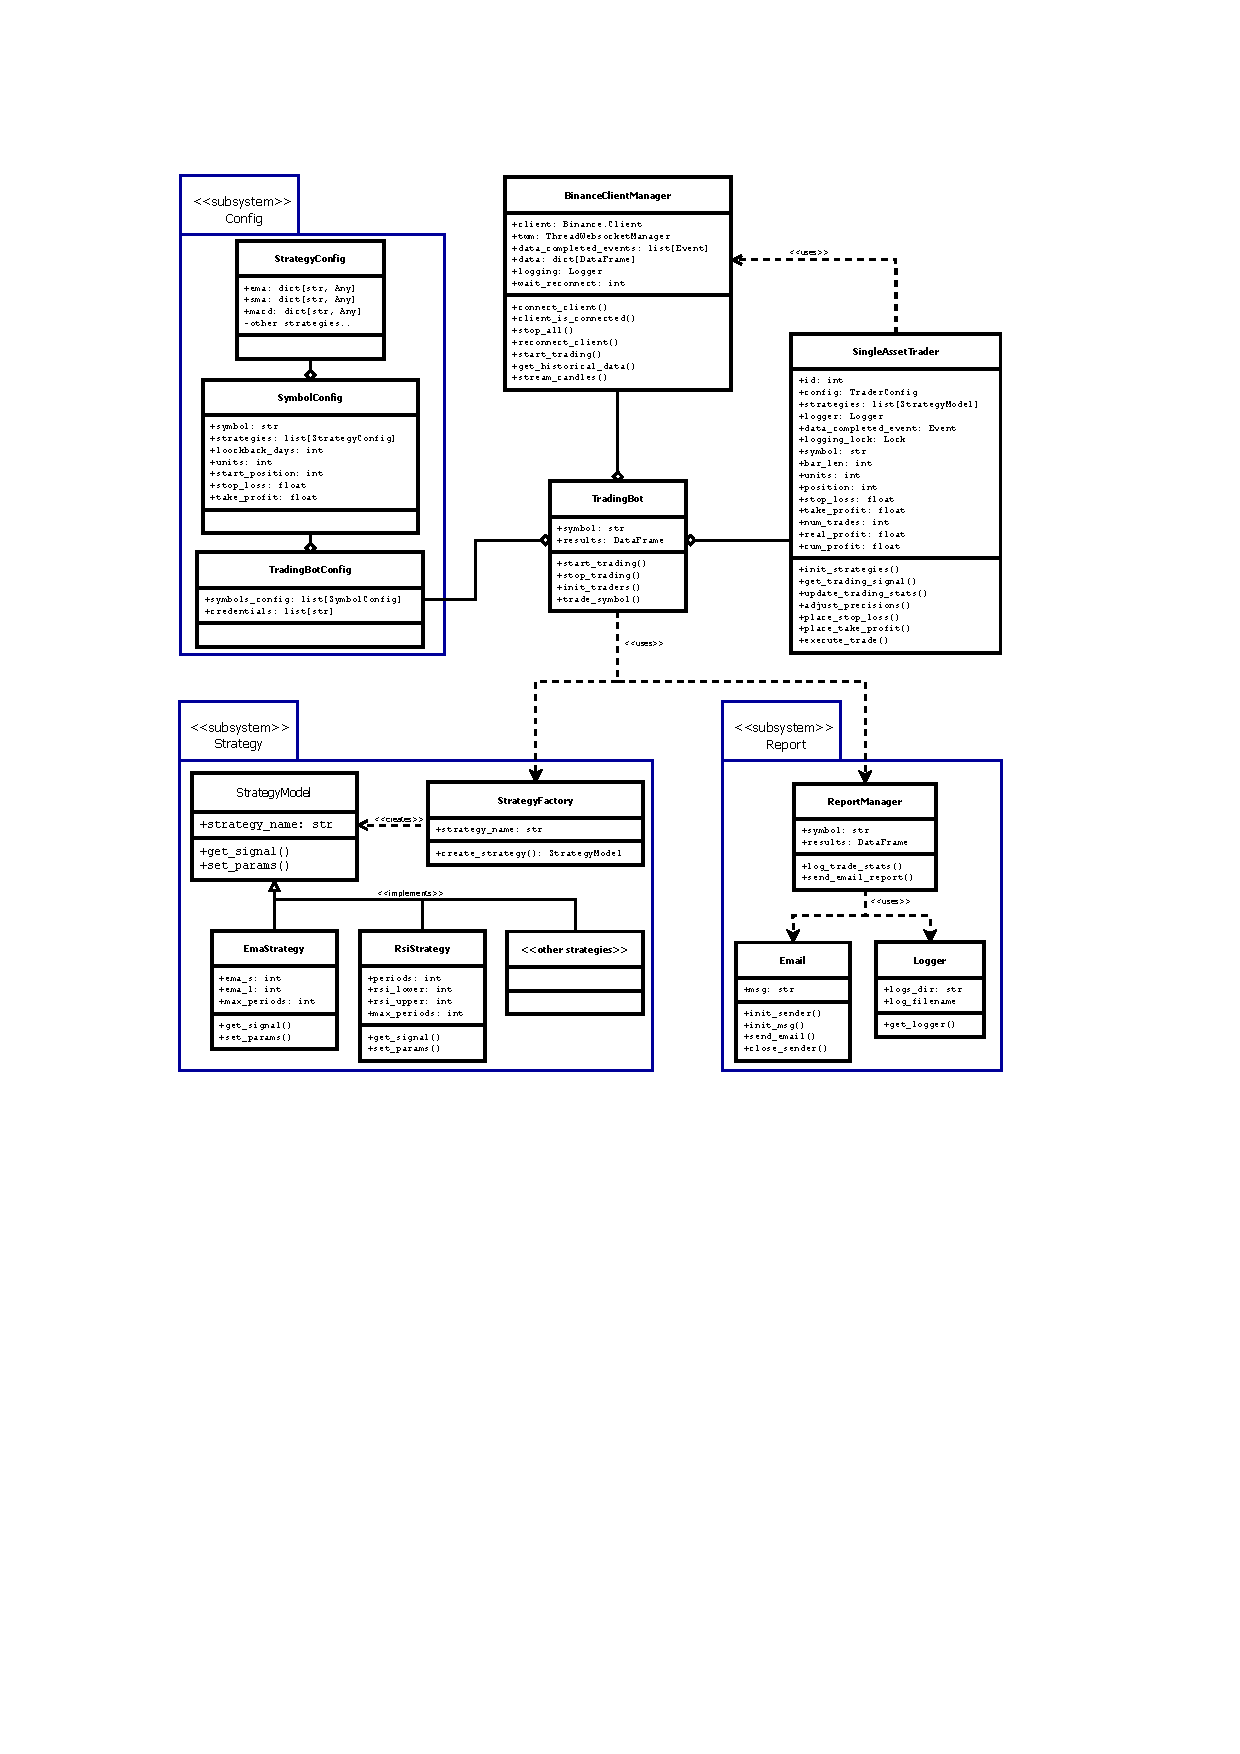
\includegraphics[page=1, trim=30mm 110mm 30mm 25mm, width=1.1\textwidth, clip]{./pdf/deployment_uml.pdf}
\caption{Architecture of the Automated Bot for Trading on the Binance Platform.}
\label{fig:deployment_arch}
\end{figure}

The deployment component of our backtesting framework is currently designed to support the Binance platform.
However, it has been architected to be extensible, allowing for potential integration with other trading platforms like Interactive Brokers for stock trading.
For any new trading platform, a dedicated client class must be provided.
In the case of Binance, all platform-specific functionalities are encapsulated within the \texttt{BinanceClientManager} class (see fig.~\ref{fig:deployment_arch}).
Any new client class should implement essential methods like \texttt{connect\_client}, \texttt{start\_trading}, \texttt{get\_historical\_data}, and \texttt{stream\_candle}.



The deployment can accommodate trading on multiple symbols using various strategies.
Since each symbol demands its specific trading details, historical data, and strategy parameters, an instance of the \texttt{SingleAssetTrader} class is created for every symbol.
This instance runs on its own dedicated thread. The \texttt{TradingManager} class ensures synchronization and coordination amongst all the components.

Configuration for trading is handled via a JSON config file.
This file specifies details like which symbols to trade on, the strategies for each symbol, their respective parameters, and more.
The \texttt{StrategyFactory} is responsible for instantiating the defined strategy models for each symbol.
These models use the retrieved historical data to generate trading signals. The \texttt{SingleAssetTrader} instances then act on these signals, placing buy or sell trades as necessary.

All trading activities are logged using a central logging system. Additionally, the framework supports email notifications for key trading events.
